\part{PDEs on Unbounded Domains}

\section{Method of characteristics}

\subsection{Well-posed Cauchy problems}
Solving partial differential equations depends on the nature of the equations in combination with the boundary or initial data.
A \vocab{Cauchy problem} is the partial differential equation for some function $\phi$ together with the auxiliary data (in $\phi$ and its derivatives) specified on a surface (or a curve in two dimensions), which is called \vocab{Cauchy data}.
For a Cauchy problem to be \textit{well-posed}, we require that
\begin{enumerate}
	\item a solution exists (we do not have excessive auxiliary data);
	\item the solution is unique (we do not have insufficient auxiliary data); and
	\item the solution depends continuously on the auxiliary data.
\end{enumerate}

\subsection{Method of characteristics}
Consider a parametrised curve $C$ given by Cartesian coordinates $(x(s), y(s))$.
The tangent vector is
\begin{align*}
	v = \qty(\dv{x(s)}{s}, \dv{y(s)}{s})
\end{align*}
We then define the directional derivative of a function $\phi(x,y)$ by
\begin{align} \label{eq:9.1}
	\eval{\dv{\phi}{s}}_C = \dv{x(s)}{s} \pdv{\phi}{x} + \dv{y(s)}{s}\pdv{\phi}{y} = v \cdot \eval{\grad{\phi}}_C
\end{align}
Suppose $v \cdot \grad{\phi} = 0$ then $\dv{\phi}{s} = 0$ and hence $\phi$ is constant along the curve. \\
Suppose there exists a vector field
\begin{align} \label{eq:9.2}
	u = \qty(\alpha(x,y), \beta(x,y))
\end{align}
with a family of non-intersecting integral curves $C$ which fill the plane (or domain of the function more generally), such that at a point $(x,y)$ the integral curve has tangent vector $u(x,y)$.

\begin{figure}[h] 
    \centering 
    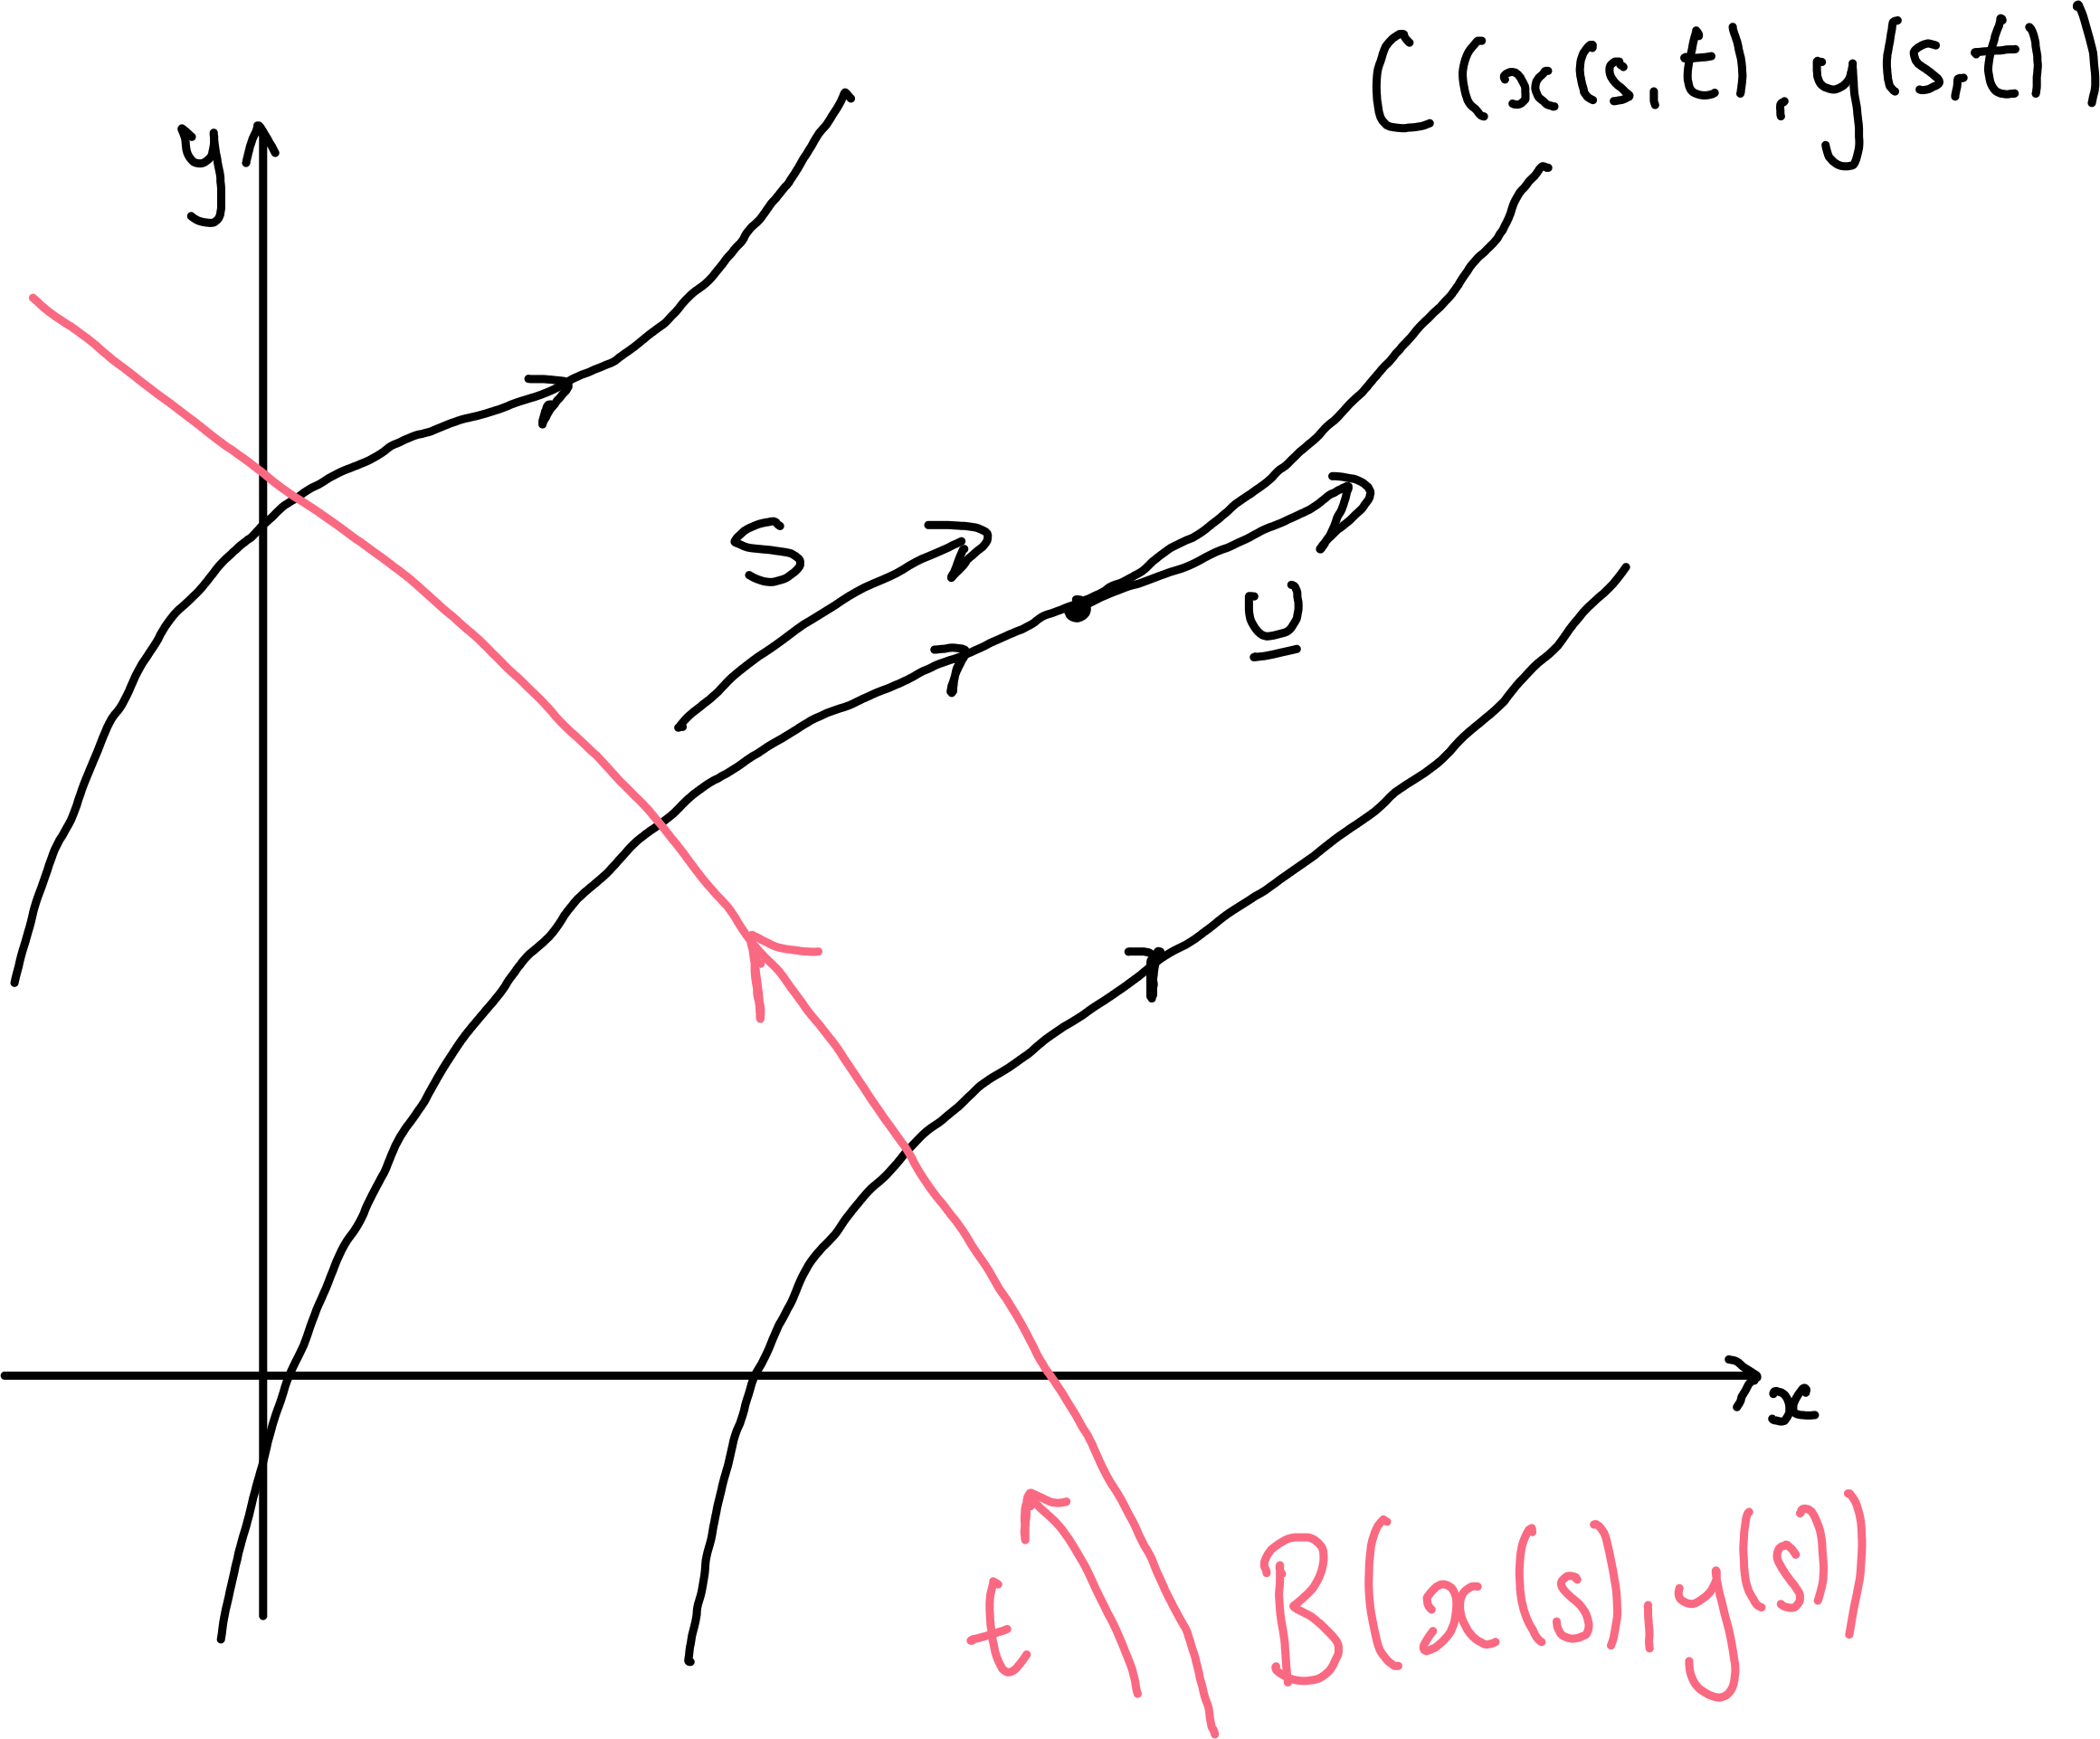
\includegraphics[height=5cm]{09-characteristicCoordinates} 
\end{figure}

Now, define a curve $B$ by $(x(t), y(t))$ such that $B$ is transverse to $u$; its tangent is nowhere parallel to $u$.
\begin{align*}
	w = \qty(\dv{x(t)}{t}, \dv{y(t)}{t}) \nparallel \qty(\alpha(x,y), \beta(x,y)) = u
\end{align*}
This can be used to parametrise the family of curves by labelling each curve $C$ with the value of $t$ at the intersection point between it and $B$.
Along the curve, we use $s$ such that $s = 0$ at the intersection.
The integral curves $(x(s,t), y(s,t))$ satisfy
\begin{align} \label{eq:9.3}
	\dv{x}{s} = \alpha(x,y);\quad \dv{y}{s} = \beta(x,y)
\end{align}
We can solve these equations to find a family of characteristic curves, along which $t$ remains constant.
This yields a new coordinate system $(s,t)$ associated with a differential equation we wish to solve.

\subsection{Characteristics of a first order PDE}
Consider
\begin{align} \label{eq:9.4}
	\alpha(x,y) \pdv{\phi}{x} + \beta(x,y) \pdv{\phi}{y} = 0
\end{align}
with Cauchy data on an initial curve $B$, defined by $(x(t), y(t))$:
\begin{align} \label{eq:9.5}
	\phi(x(t), y(t)) = f(t)
\end{align}
Note,
\begin{align*}
	\alpha \phi_x + \beta \phi_y = u \cdot \grad{\phi} = \eval{\dv{\phi}{s}}_C
\end{align*}
This is exactly the directional derivative along the integral curve $C$, defined by $u = (\alpha, \beta)$, which are called the \vocab{characteristic curves of the PDE}.
Since $\dv{\phi}{s} = \alpha \phi_x + \beta \phi_y = 0$ from the original PDE \cref{eq:9.4}, the function $\phi(x,y)$ is constant along this curve $C$.
In other words, the Cauchy data $f(t)$ defined on $B$ at $s = 0$ is propagated constantly along the integral curves.
This gives the solution
\begin{align} \label{eq:9.6}
	\phi(s,t) = \phi(x(s,t), y(s,t)) = f(t)
\end{align}
To obtain $\phi$ in the original coordinates, we need to transform from $s,t$-space into $x,y$-space.
Provided that the Jacobian $J = x_t y_s - x_s y_t$ is nonzero, we can invert the transformation and find $s,t$ as functions of $x,y$.
This gives
\begin{align} \label{eq:9.7}
	\phi(x,y) = f(t(x,y))
\end{align}
To solve such a PDE i.e. \cref{eq:9.4} given \cref{eq:9.5}, we will typically use the following steps.
\begin{enumerate}
	\item Find the characteristic equations \cref{eq:9.3}, $\dv{x}{s} = \alpha, \dv{y}{s} = \beta$.
	\item Parametrise the initial conditions on 
    \begin{align} \label{eq:9.8}
        B(x(t), y(t))
    \end{align}
	\item Solve the characteristic equations to find $x = x(s,t)$ and $y = y(s,t)$ subject to the initial conditions, \cref{eq:9.8}, at $s = 0$.
	\item Solve the equation for $\phi$, \cref{eq:9.4} with \cref{eq:9.1}, given by $\dv{\phi}{s} = \alpha \phi_x + \beta \phi_y = 0$, so $\phi$ is constant along the integral curves, giving $\phi(s,t) = f(t)$, \cref{eq:9.6}.
	\item Invert the relations $s = s(x,y)$ and $t = t(x,y)$, then find $\phi$ in terms of $x,y$.
\end{enumerate}

\begin{example}
	Consider the equation
	\begin{align*}
		\dv{\phi(x,y)}{x} = 0
	\end{align*}
	such that
	\begin{align*}
		\phi(0,y) = h(y)
	\end{align*}

    \begin{enumerate}
        \item The characteristic equations are given by
        \begin{align*}
            \dv{x}{s} = \alpha = 1;\quad \dv{y}{s} = \beta = 0 \tag{$\ast$}
        \end{align*}
        \item The initial curve $B$ is given by
        \begin{align*}
            (x(t), y(t)) = (0,t) \tag{$\dagger$}
        \end{align*}
        \item Solving the characteristic equations $(\ast)$,
        \begin{align*}
            x = s + c(t);\quad y = d(t)
        \end{align*}
        At $x = 0$, we must have $s = 0$, so $c = 0$.
        Further, $y = t$ hence $d = t$.
        Thus,
        \begin{align*}
            x = s;\quad y = t
        \end{align*}
        \item Thus,
        \begin{align*}
            \dv{\phi}{x} = 0 \implies \phi(s,t) = h(t) \implies \phi(x,y) = h(y)
        \end{align*}
    \end{enumerate} 
\end{example}

\begin{example}
	Consider
	\begin{align*}
		e^x \phi_x + \phi_y = 0;\quad \phi(x,0) = \cosh x
	\end{align*}
    \begin{enumerate}
        \item The characteristic equations are
        \begin{align*}
            \dv{x}{s} = e^x;\quad \dv{y}{s} = 1 \tag{$\ast$}
        \end{align*}
        \item The initial conditions are
        \begin{align*}
            x(t) = t;\quad y(t) = 0 \tag{$\dagger$}
        \end{align*}
        We solve the characteristic equation subject to these initial conditions, giving
        \begin{align*}
            -e^{-x} = s + c(t);\quad y = s + d(t)
        \end{align*}
        $s = 0$ ($x = t$) implies $-e^{-t} = c(t)$ and $y = 0 = d(t)$.
        Hence
        \begin{align*}
            e^{-x} = e^{-t} - s;\quad y = s
        \end{align*}
        \item Now,
        \begin{align*}
            \dv{\phi}{s} = 0 \implies \phi(s,t) = \cosh t
        \end{align*}
        \item Since $s = y, e^{-t} = y + e^{-x}$, we have $t = -\log(y + e^{-x})$.
        Thus,
        \begin{align*}
            \phi(x,y) = \cosh\qty[-\log(y + e^{-x})]
        \end{align*}
    \end{enumerate} 

\end{example}

\subsection{Inhomogeneous first order PDEs}
Suppose we now wish to solve
\begin{align} \label{eq:9.9}
	\alpha(x,y) \phi_x + \beta(x,y) \phi_y = \gamma(x,y)
\end{align}
with Cauchy data $\phi(x(t), y(t)) = f(t)$ along a curve $B$.
The characteristic curves are the same as the homogeneous case \cref{eq:9.4}.
However, the directional derivative no longer vanishes:
\begin{align} \label{eq:9.10}
	\eval{\dv{\phi}{s}}_C = u \cdot \grad{\phi} = \gamma(x,y)
\end{align}
where $\phi = f(t)$ at $s = 0$ on $B$.
So $f(t)$ is no longer propagated constantly across characteristic polynomials, but is instead propagated according to the ODE in $s$ \cref{eq:9.10}.
We must therefore solve this ODE along $C$ before reverting to $x,y$ coordinates.

\begin{example}
	Consider
	\begin{align*}
		\phi_x + 2 \phi_y = ye^x;\quad \phi(x,x) = \sin x
	\end{align*}
    \begin{enumerate}
        \item The characteristic equation is given by
        \begin{align*}
            \dv{x}{s} = 1;\quad \dv{y}{s} = 2 \tag{$\ast$}
        \end{align*}
        \item The initial conditions are
        \begin{align*}
            x(t) = y(t) = t \tag{$\dagger$}
        \end{align*}
        \item From the characteristic equations,
        \begin{align*}
            x = s + c(t);\quad y = 2s + d(t)
        \end{align*}
        Thus when $s = 0$ $(\dagger)$ implies,
        \begin{align*}
            x = t = c(t);\quad y = t = d(t)
        \end{align*}
        So the solutions to the characteristics are
        \begin{align*}
            x = s + t;\quad y = 2s + t
        \end{align*}
        \item Now we solve
        \begin{align*}
            \dv{\phi}{s} = \gamma = y e^x = (2s+t)e^{s+t}
        \end{align*}
        Note that $\dv{s} \qty(2se^s) = 2e^s + 2se^s$, so the solution is
        \begin{align*}
            \phi(s,t) = (2s - 2 + t)e^{s+t} + c(s)
        \end{align*}
        for some constant term $c(s)$.
        But $\phi(0,t) = \sin t$, hence
        \begin{align*}
            \sin t = (t-2)e^t + c(s) \implies \phi(s,t) = (2s-2+t)e^{s+t} + \sin t + (2-t)e^t
        \end{align*}
        \item Inverting into $x,y$ space, since $s = y - x$, $t = 2x - y$,
        \begin{align*}
            \phi(x,y) = (y-2)e^x + (y-2x+2)e^{2x-y} + \sin(2x-y)
        \end{align*}
    \end{enumerate} 
\end{example}

\subsection{Classification of second order PDEs}
In two dimensions, the general second order PDE is
\begin{align} \label{eq:9.11}
    \begin{split}
        \mathcal L \phi & \equiv a(x,y) \pdv[2]{\phi}{x} + 2 b(x,y) \pdv{\phi}{x}{y} + c(x,y) \pdv[2]{\phi}{y} \\
        &+ d(x,y) \pdv{\phi}{x} + e(x,y) \pdv{\phi}{y} + f(x,y) \phi(x,y)
    \end{split} 
\end{align}
The \textit{principal part} is given by
\begin{align*}
	\sigma_P (x,y,k_x,k_y) \equiv k^T A k = \begin{pmatrix}
		k_x & k_y
	\end{pmatrix} \begin{pmatrix}
		a(x,y) & b(x,y) \\
		b(x,y) & c(x,y)
	\end{pmatrix} \begin{pmatrix}
		k_x \\ k_y
	\end{pmatrix}
\end{align*}
The PDE is classified by the properties of the eigenvalues of $A$.
\begin{enumerate}
	\item If $b^2 - ac < 0$, the equation is \textit{elliptic}.
	      The eigenvalues have the same sign.
	      An example is the Laplace equation, \cref{eq:5.1}.
	\item If $b^2 - ac > 0$, the equation is \textit{hyperbolic}.
	      The eigenvalues have opposite signs.
	      An example is the wave equation, \cref{eq:3.4}.
	\item If $b^2 - ac = 0$, the equation is \textit{parabolic}, where at least one eigenvalue is zero.
	      An example is the heat equation, \cref{eq:4.3}.
\end{enumerate}
Note that a differential equation may have different classifications at different points $(x,y)$ in space.

\subsection{Characteristic curves of second order PDEs}
A curve defined by $f(x,y) =$ constant is a characteristic if
\begin{align} \label{eq:9.12}
	\begin{pmatrix}
		f_x & f_y
	\end{pmatrix} \begin{pmatrix}
		a & b \\
		b & c
	\end{pmatrix} \begin{pmatrix}
		f_x \\ f_y
	\end{pmatrix} = 0
\end{align}
This is a generalisation of the first order case $u \cdot \grad{f} = 0$ where $u = (\alpha, \beta)$.
The curve can be written as $y = y(x)$ by the chain rule.
\begin{align} \label{eq:9.13}
	\pdv{f}{x} + \pdv{f}{y} \dv{y}{x} = 0 \implies \frac{f_x}{f_y} = -\dv{y}{x}
\end{align}
Substituting into the quadratic form \cref{eq:9.12},
\begin{align*}
	a \qty(\dv{y}{x})^2 - 2b \dv{y}{x} + c = 0
\end{align*}
for which we have a quadratic solution given by
\begin{align} \label{eq:9.14}
	\dv{y}{x} = \frac{b \pm \sqrt{b^2 - ac}}{a}
\end{align}
\begin{enumerate}
	\item Hyperbolic equations have two such solutions, since $b^2 - ac > 0$.
	\item Parabolic equations have one solution.
	\item Elliptic equations have no real characteristics.
\end{enumerate}

\subsection{Characteristic coordinates}
Transforming to characteristic coordinates $u,v$ will set $a = 0$ and $c = 0$ in \cref{eq:9.11}.
Hence, the PDE will take the \vocab{canonical form}
\begin{align} \label{eq:9.15}
	\pdv{\phi}{u}{v} + \dots + = 0
\end{align}
where the omitted terms are lower order, e.g. $\phi_u, \phi_v, \phi \dots$

\begin{example}
	Consider
	\begin{align*}
		-y \phi_{xx} + \phi_{yy} = 0 \tag{$\ast$}
	\end{align*}
	Here, $a = -y, b = 0, c = 1$ hence $b^2 - ac = y$.
	For $y > 0$, the equation is hyperbolic, for $y < 0$ it is elliptic, and for $y = 0$ it is parabolic.
	Consider the characteristics for $y > 0$.
	\begin{align*}
		\dv{y}{x} = \frac{b \pm \sqrt{b^2 - ac}}{a} = \pm \frac{1}{\sqrt{y}}
	\end{align*}
	Hence,
	\begin{align*}
		\int \sqrt{y} \dd{y} = \pm \int \dd{x} \implies \frac{2}{3} y^{\frac{3}{2}} \pm x = C_\pm
	\end{align*}
	Therefore, the characteristic curves are
	\begin{align*}
		u = \frac{2}{3} y^{\frac{3}{2}} + x;\quad v = \frac{2}{3} y^{\frac{3}{2}} - x
	\end{align*}
	Taking derivatives,
	\begin{align*}
		u_x = 1;\quad u_y = \sqrt{y};\quad v_x = -1;\quad v_y = \sqrt{y}
	\end{align*}
	Hence,
	\begin{align*}
		\phi_x &= \phi_u u_x + \phi_v v_x = \phi_u - \phi_v \\
		\phi_y &= \sqrt{y} (\phi_u + \phi_v) \\
		\phi_{xx} &= \phi_{uu} - 2 \phi_{uv} + \phi_{vv} \\
		\phi_{yy} &= y (\phi_{uu} + 2 \phi_{uv} + \phi_{vv}) + \frac{1}{2\sqrt{y}}(\phi_u + \phi_v)
	\end{align*}
	Substituting into the original PDE ($\ast$),
	\begin{align*}
		-y \phi_{xx} + \phi_{yy} = y\qty(4 \phi_{uv} + \frac{1}{2y^{\frac{3}{2}}} (\phi_u + \phi_v) )
	\end{align*}
	Note, $u + v = \frac{4}{3} y^{\frac{3}{2}}$, hence we have the canonical form
	\begin{align*}
		4 \phi_{uv} + \frac{1}{6(u+v)} (\phi_u + \phi_v) = 0
	\end{align*}
\end{example}

\subsection{General solution to wave equation}
The wave equation, \cref{eq:3.4}, is
\begin{align*}
	\frac{1}{c^2} \pdv[2]{\phi}{t} - \pdv[2]{\phi}{x} = 0
\end{align*}
We wish to solve this with initial conditions
\begin{align} \label{eq:9.16}
	\phi(x,0) = f(x),\quad \phi_t(x,0) = g(x)
\end{align} 
Here, $a = \frac{1}{c^2}, b = 0, c = -1$ hence $b^2 - ac > 0$.
The characteristic equation is
\begin{align*}
	\dv{x}{t} = \frac{0 \pm \sqrt{0 + \frac{1}{c^2}}}{\frac{1}{c^2}} = \pm c
\end{align*}
Hence the characteristic coordinates are
\begin{align*}
	u = x - ct;\quad v = x + ct
\end{align*}
This yields the canonical form
\begin{align} \label{eq:9.17}
	\pdv{\phi}{u}{v} = 0
\end{align}
This may be integrated directly to find
\begin{align*}
	\pdv{\phi}{v} = F(v) \implies \phi = G(u) + \int^v F(y) \dd{y} = G(u) + H(v)
\end{align*}
Imposing the initial conditions at $t = 0$, we find $u = v = x$ and
\begin{align*}
	G(x) + H(x) = f(x);\quad -cG'(x) + cH'(x) = g(x)
\end{align*}
Differentiating the first equation, we find
\begin{align*}
	G'(x) + H'(x) = f'(x)
\end{align*}
We can combine this with the second equation to give
\begin{align*}
	H'(x) = \frac{1}{2} \qty(f'(x) + \frac{1}{c}g(x)) \implies H(x) = \frac{1}{2} \qty(f(x) - f(0)) + \frac{1}{2c}\int_0^x g(y) \dd{y}
\end{align*}
Similarly,
\begin{align*}
	G'(x) = \frac{1}{2} \qty(f'(x) - \frac{1}{c}g(x)) \implies G(x) = \frac{1}{2} \qty(f(x) - f(0)) - \frac{1}{2c}\int_0^x g(y) \dd{y}
\end{align*}
The final solution is therefore
\begin{align} \label{eq:9.18}
	\phi(x,t) = G(x-ct) + H(x+ct) = \frac{1}{2}\qty(f(x-ct) + f(x+ct)) + \frac{1}{2c} \int_{x-ct}^{x+ct} g(y) \dd{y}
\end{align}

\underline{Domain of dependence} \\
Waves propagate at a velocity $c$, hence $\phi(x,t)$ is fully determined by values of $f, g$ in the interval $[x-ct, x+ct]$.
This is the same idea as light cones in special relativity.